\documentclass[hide notes,intlimits]{beamer}

\mode<presentation>
{
  \usetheme[footline]{PISMshade}
  \setbeamercovered{transparent}
}

\usepackage{pgfpages}

\usepackage{verbatim,amsmath,empheq,times,bm}
\usepackage[english]{babel}
\usepackage[utf8]{inputenc}

\usepackage{tikz}
\usepackage{animate}
\usepackage{hyperref}

\definecolor{dark red}{HTML}{E41A1C}
\definecolor{dark green}{HTML}{4DAF4A}
\definecolor{dark violet}{HTML}{984EA3}
\definecolor{dark blue}{HTML}{084594}
\definecolor{dark orange}{HTML}{FF7F00}
\definecolor{light blue}{HTML}{377EB8}
\definecolor{light red}{HTML}{FB9A99}
\definecolor{light violet}{HTML}{CAB2D6}

\setbeamercolor{boxed}{fg=black,bg=uaf yellow}

\newcommand{\CC}{\mathbb{C}}
\newcommand{\NN}{\mathbb{N}}
\newcommand{\RR}{\mathbb{R}}
\newcommand{\ZZ}{\mathbb{Z}}
\newcommand{\Acal}{\mathcal{A}}
\newcommand{\Bcal}{\mathcal{B}}
\newcommand{\Ccal}{\mathcal{C}}
\newcommand{\Ncal}{\mathcal{N}}
\newcommand{\Kcal}{\mathcal{K}}

\newcommand{\bF}{\mathbf{F}}
\newcommand{\bQ}{\mathbf{Q}}
\newcommand{\bU}{\mathbf{U}}

\newcommand{\bbU}{\bar{\bU}}

\newcommand{\bb}{\mathbf{b}}
\newcommand{\bu}{\mathbf{u}}
\newcommand{\bv}{\mathbf{v}}
\newcommand{\bx}{\mathbf{x}}

\newcommand{\Div}{\nabla\cdot}
\newcommand{\eps}{\epsilon}
\newcommand{\grad}{\nabla}
\newcommand{\lap}{\triangle}
\DeclareMathOperator{\trace}{tr}
\renewcommand{\bar}{\overline}

\newcommand{\ddx}[1]{\frac{\partial #1}{\partial x}}
\newcommand{\ddy}[1]{\frac{\partial #1}{\partial y}}
\newcommand{\pp}[2]{\frac{\partial #1}{\partial #2}}
\newcommand{\ppt}[1]{\frac{\partial #1}{\partial t}}
\newcommand{\ppT}[1]{\frac{\partial #1}{\partial T}}
\newcommand{\ppx}[1]{\frac{\partial #1}{\partial x}}
\newcommand{\ppy}[1]{\frac{\partial #1}{\partial y}}
\newcommand{\ppz}[1]{\frac{\partial #1}{\partial z}}
\newcommand{\ppxx}[1]{\frac{\partial^2 #1}{\partial x^2}}
\newcommand{\ppzz}[1]{\frac{\partial^2 #1}{\partial z^2}}

\newcommand{\Tnorm}[1]{\left|\!\left|\!\left|#1\right|\!\right|\!\right|}
\newcommand{\rhow}{\rho_{\text{w}}}
\newcommand{\Wq}{W^{1,q}(\Omega)}
\newcommand{\half}{\frac12}

%\setbeamercolor{redtext}{fg=red!80!black}
\setbeamercolor{redtext}{fg=red!94!black}
%\setbeamercolor{greentext}{fg=green!80!black}
\setbeamercolor{greentext}{fg=green!60!black}
%\setbeamercolor{bluetext}{fg=blue!70!black}
\setbeamercolor{bluetext}{fg=blue!90!black}
\setbeamercolor{yellowtext}{fg=yellow!95!black}
\setbeamercolor{orangetext}{fg=yellow!50!red}

\newcommand{\green}{\usebeamercolor[fg]{greentext}}
\newcommand{\blue}{\usebeamercolor[fg]{bluetext}}
\newcommand{\red}{\usebeamercolor[fg]{redtext}}

\renewcommand{\L}{\emph{Left}}
\newcommand{\R}{\emph{Right}}


\newcommand{\contactslipslide}{
\begin{frame}{sheets vs.~streams vs.~shelves}

\begin{columns}
\begin{column}{0.35\textwidth}
\small
\begin{itemize}
\small
\item non-sliding portions of ice sheets flow by shear deformation
\item ice streams slide: \alert{contact slip}
\item ``ice shelves'' are floating thick ice
  \begin{itemize}
  \scriptsize
  \item[$\circ$] also \alert{contact slip}
  \end{itemize}
\end{itemize}
\end{column}

\begin{column}{0.65\textwidth}

\hfill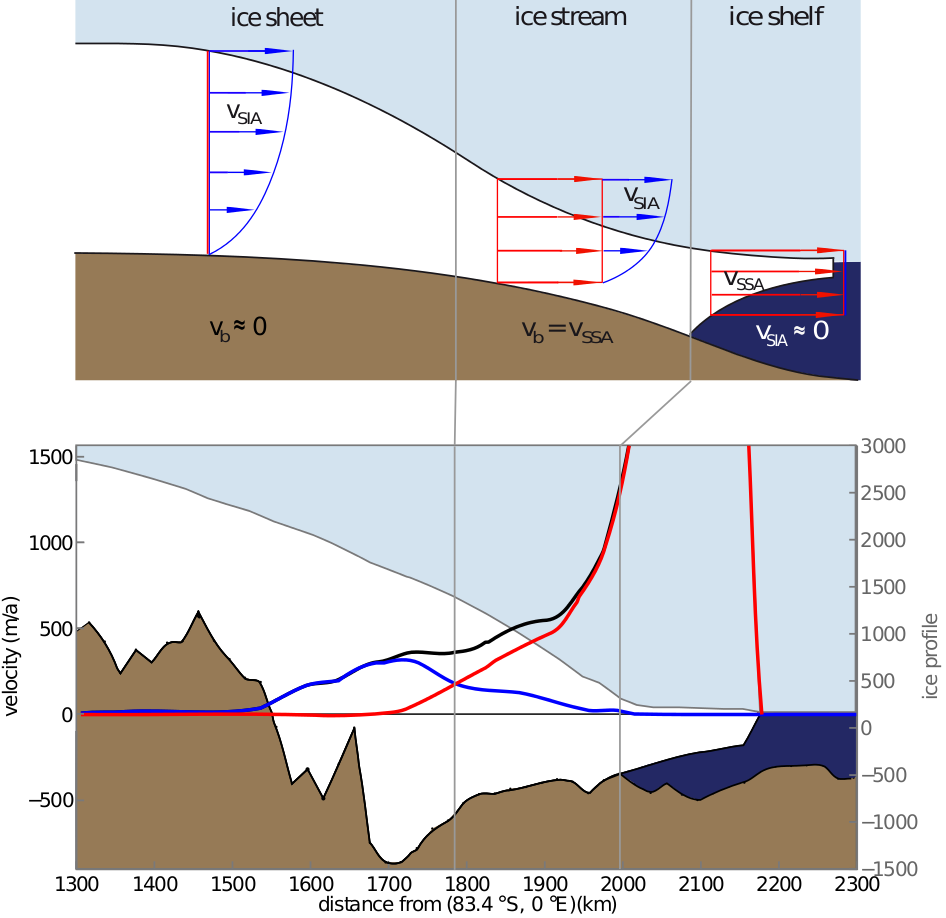
\includegraphics[width=0.95\textwidth]{siassacartoon-lambert}

\begin{center}
\vspace{-0.18in}
\tiny [Lambert glacier and Amery ice shelf, Antarctic]
\end{center}
\end{column}
\end{columns}
\end{frame}
}



\title{Flowing ice in glaciers and ice sheets \\ (as applied math)}

\author[Bueler]{Ed Bueler}

\institute[UAF]{
  \tiny Dept of Mathematics and Statistics \\

  University of Alaska Fairbanks
}

\date{\tiny 18 May, 2018}


\setbeamerfont{date}{size=\scriptsize}

\subject{ice sheets, glaciers, numerical analysis, applied mathematics}


\AtBeginSection[]
{
  \begin{frame}<beamer>
    \frametitle{Outline}
    \tableofcontents[currentsection,hideallsubsections]
  \end{frame}
}


\begin{document}
\graphicspath{{../../old/commonfigs/}{../../figures/}}

\begin{frame}
  \titlepage
  \begin{center}
  \tiny supported by NASA grants NNX13AM16G, NNX16AQ40G, NNX17AG65G 
  \end{center}
\end{frame}



% NO OUTLINE BECAUSE ONE APPEARS AT START OF EACH SECTION ?
%\begin{frame}
  %\frametitle{Outline}
  %\tableofcontents[hideallsubsections]
  % You might wish to add the option [pausesections]
%\end{frame}


\section[the alien view]{the alien physicist view of Greenland}

\setbeamertemplate{background canvas}{
     \tikz{\node[inner sep=0pt,opacity=1] {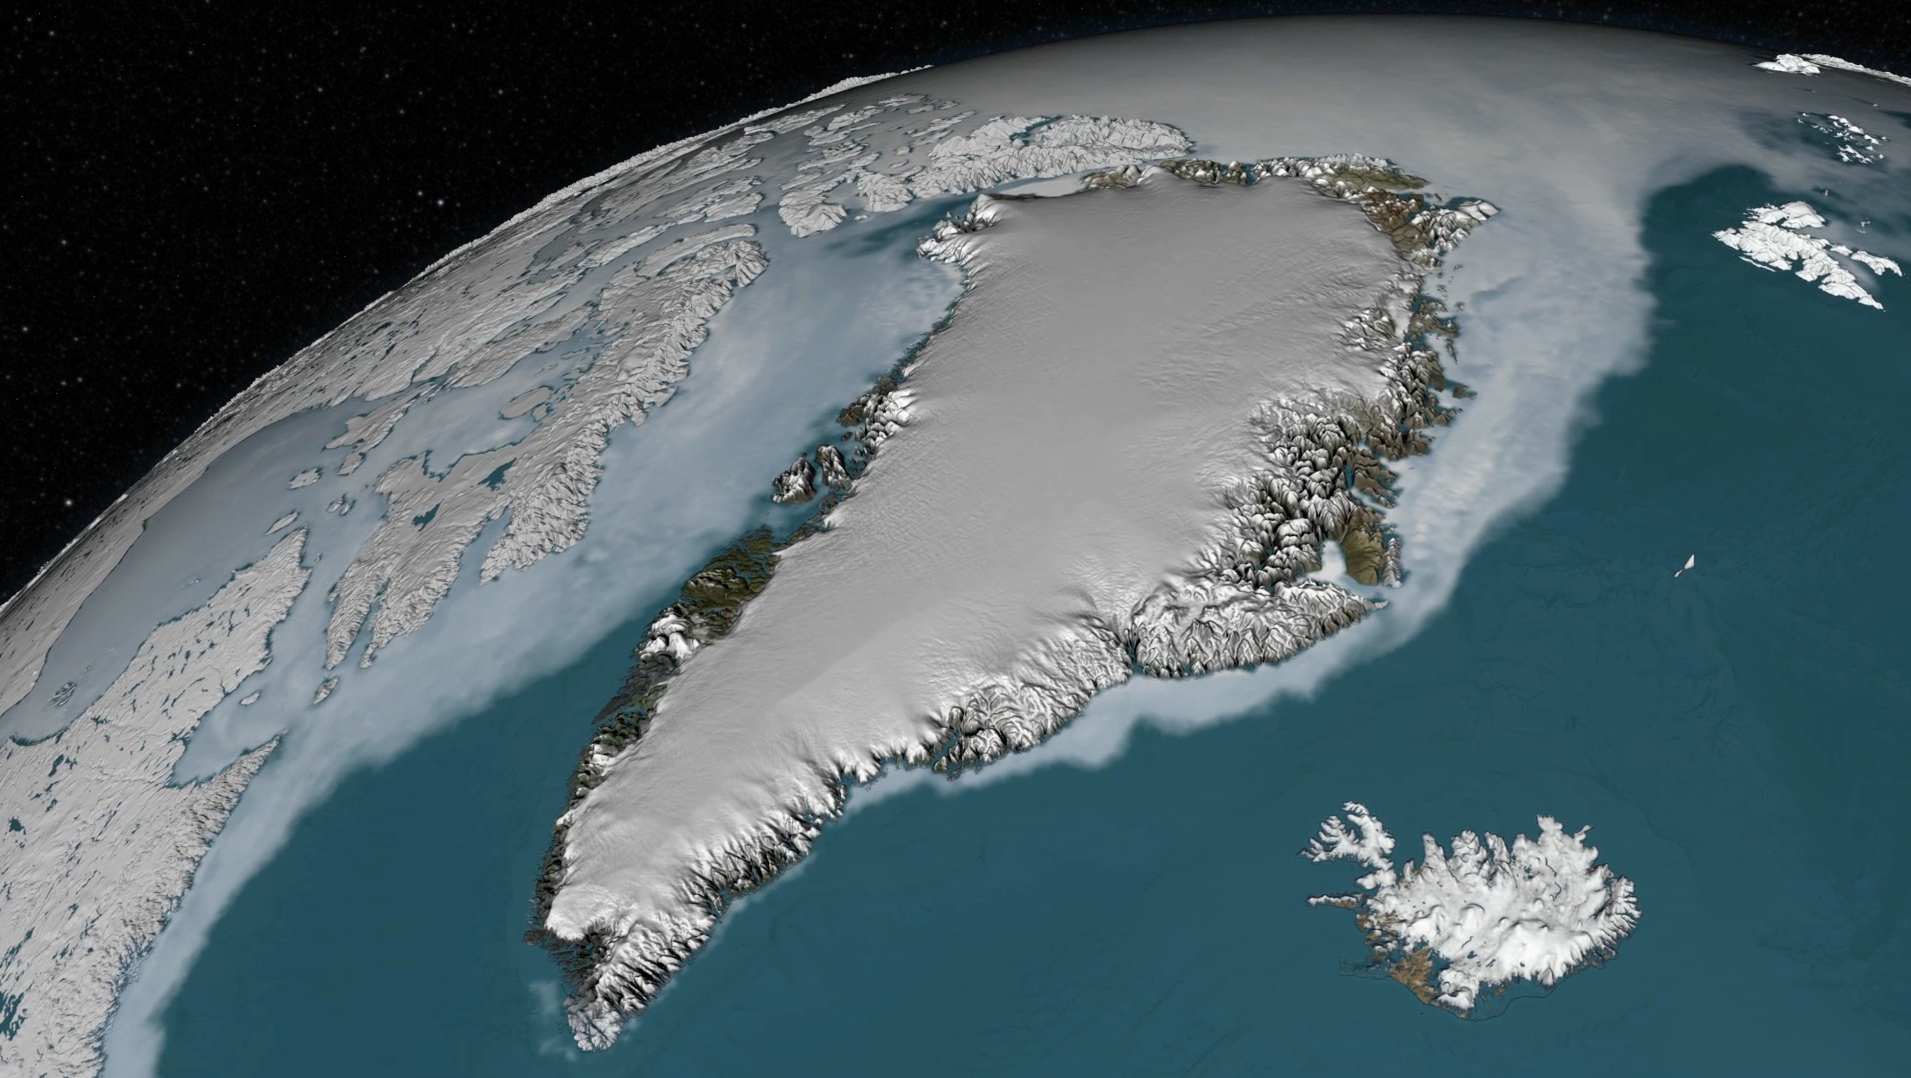
\includegraphics[height=\paperheight,width=\paperwidth]{nasa-mapping-greenland-ice-sheet}};}
} 

\begin{frame}{}

\only<2>{
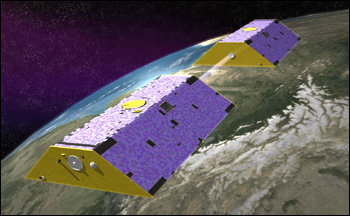
\includegraphics[width=0.3\textwidth]{grace-satellites}

\vfill \hfill 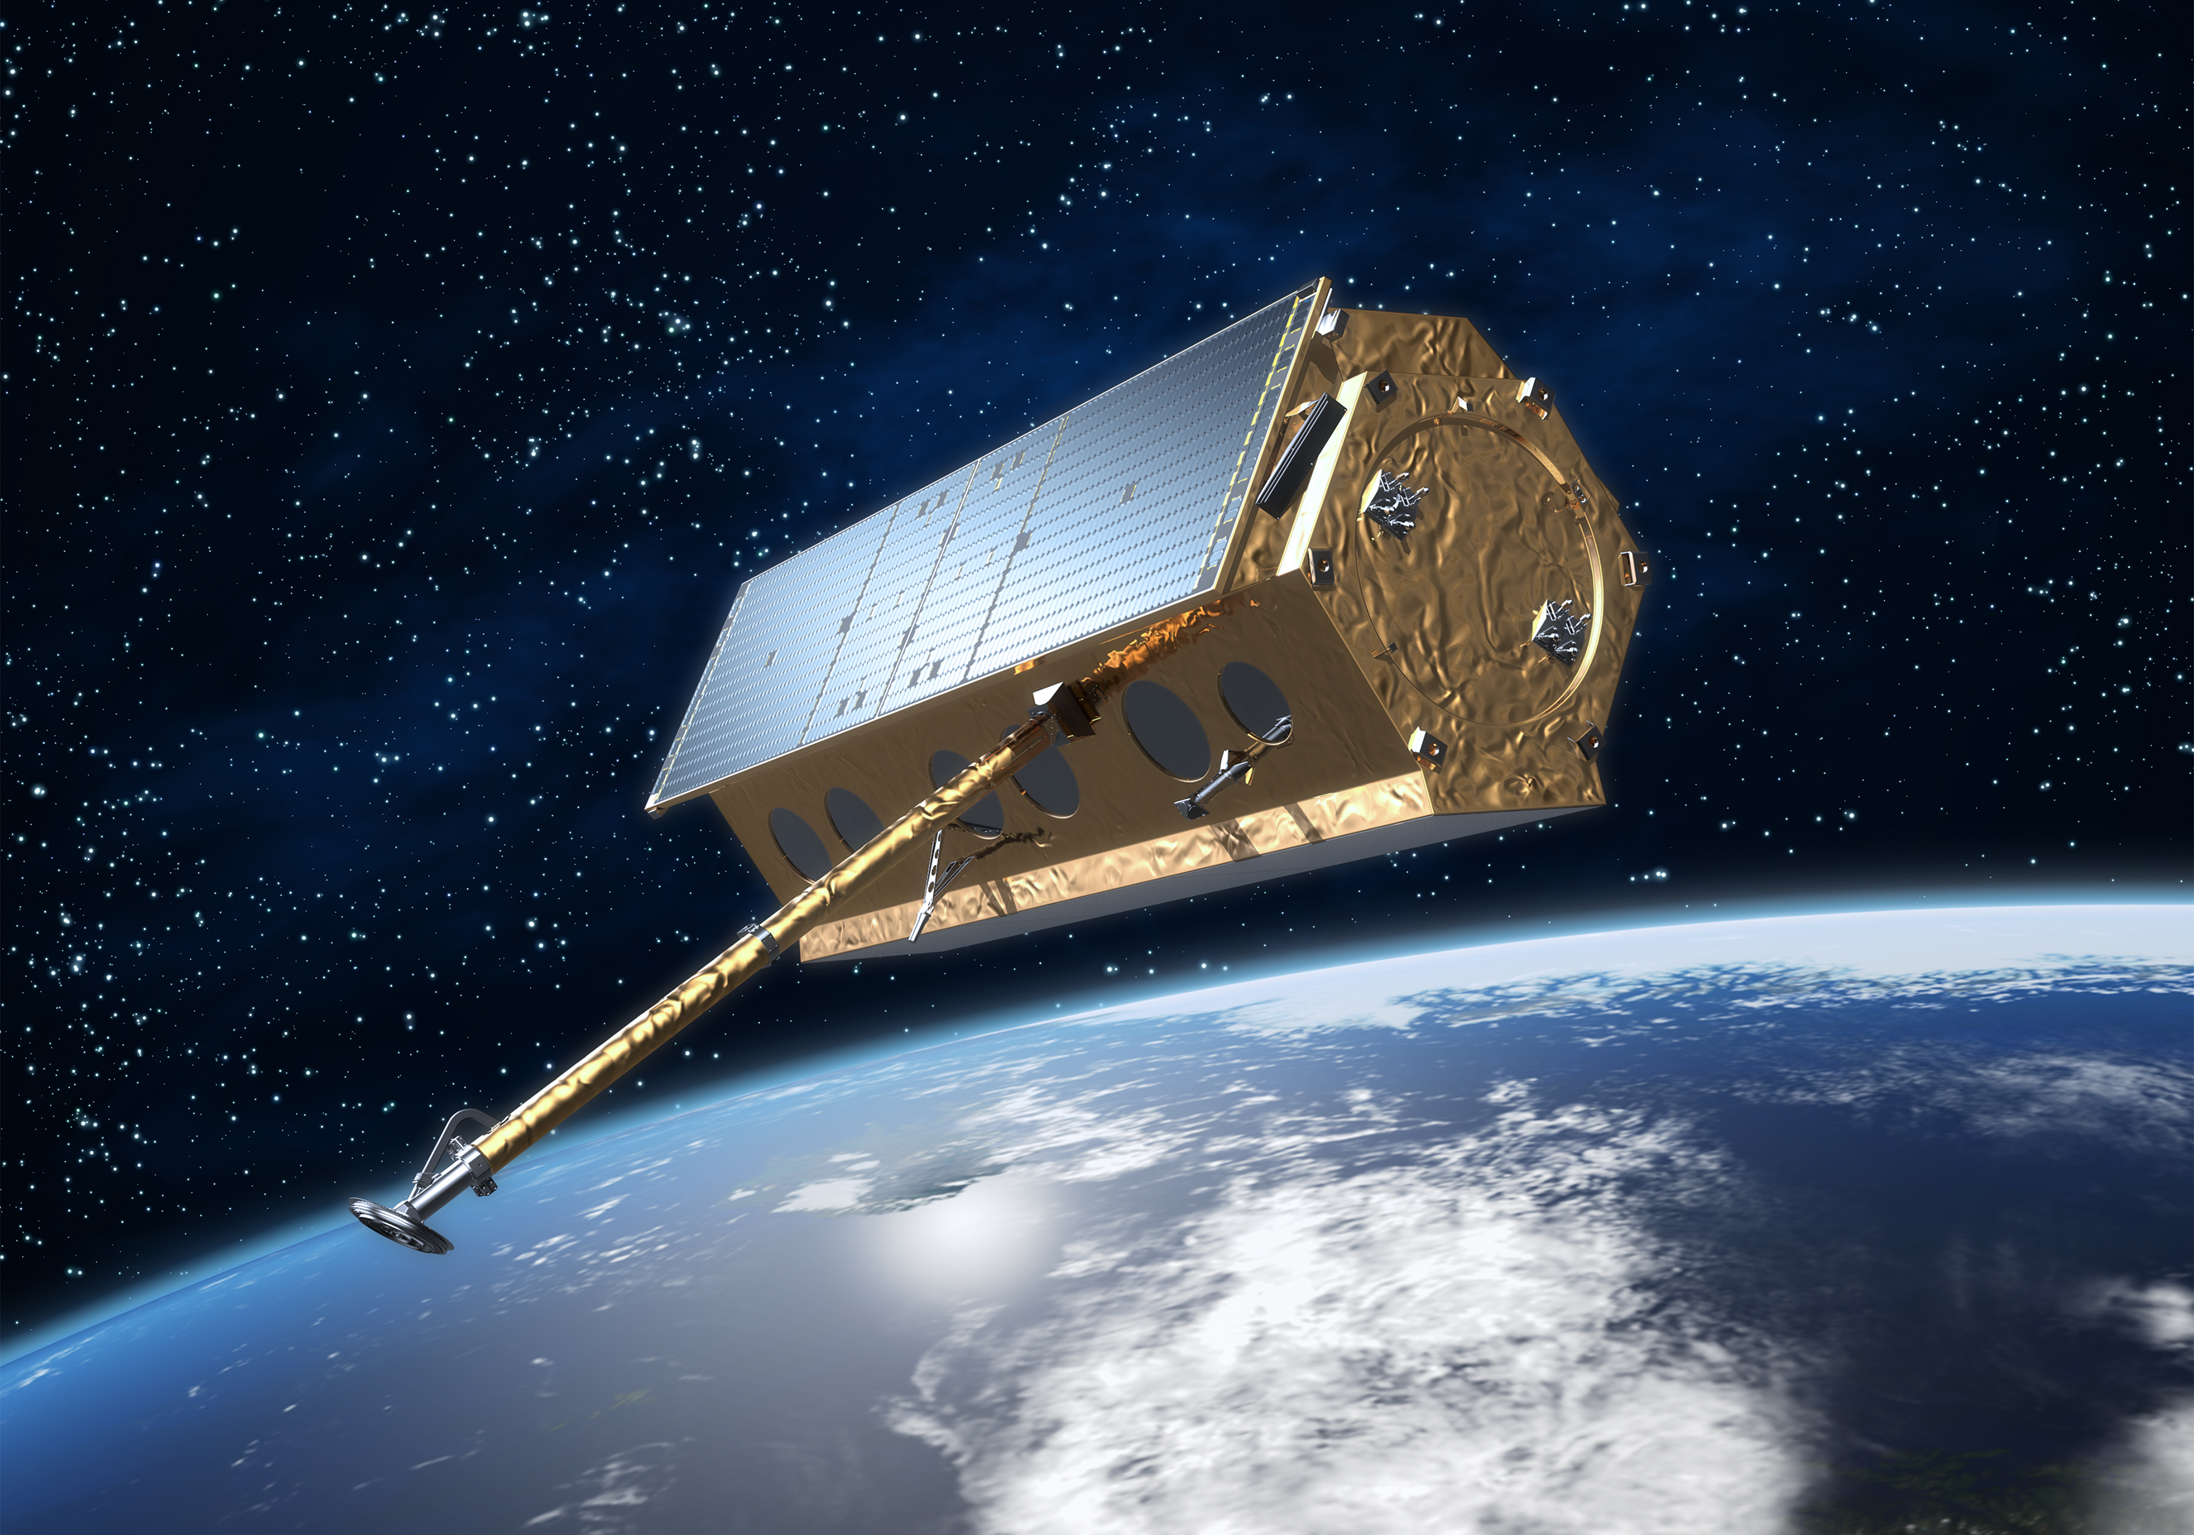
\includegraphics[width=0.3\textwidth]{TerraSAR_n}
}
\end{frame}


\setbeamertemplate{background canvas}{}

\begin{frame}{the view from space}

\begin{columns}
\begin{column}{0.6\textwidth}
\begin{itemize}
\item satellites can measure gravity changes \hfill \alert{\dots show GRACE movie}
\item satellites can measure movement of earth surface through \emph{synthetic aperture radar} (SAR) \hfill \alert{\dots at right}
\end{itemize}
\end{column}
\begin{column}{0.4\textwidth}

\hfill 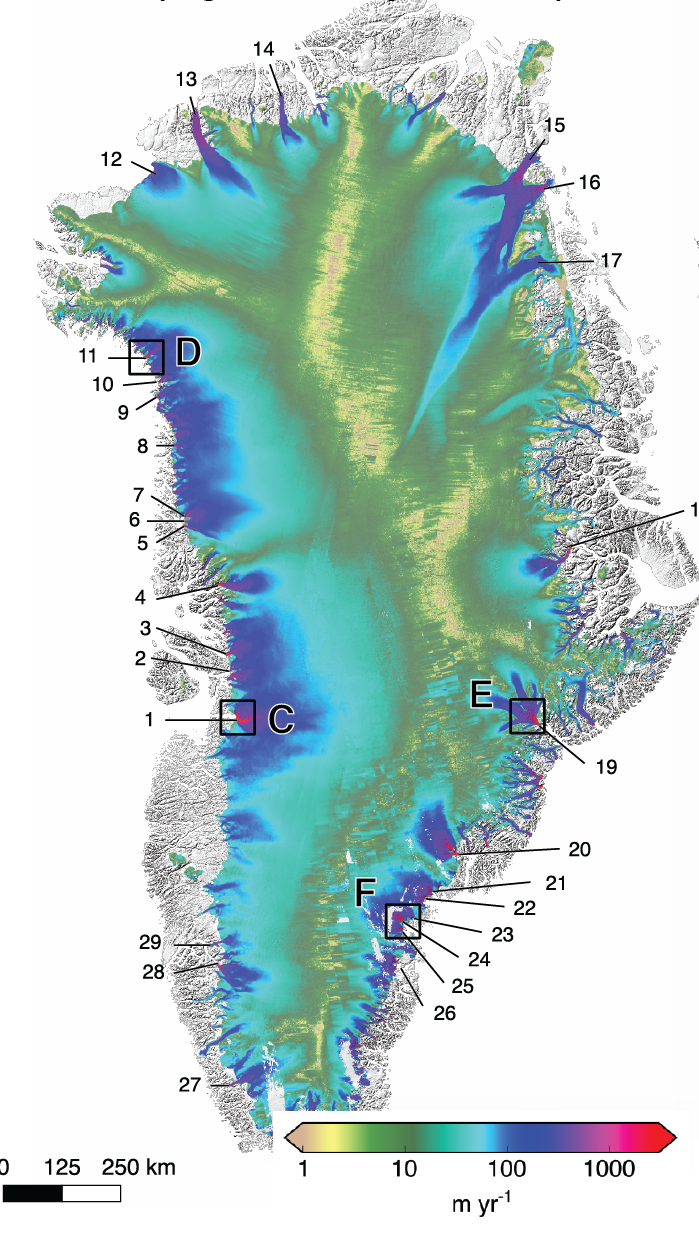
\includegraphics[width=0.95\textwidth]{greenland-overview-obsonly}
\end{column}
\end{columns}
\end{frame}


\section[intro to ice flow]{an introduction to flowing ice}


\begin{frame}{ice in glaciers is a viscous fluid}
\begin{columns}
\begin{column}{0.65\textwidth}
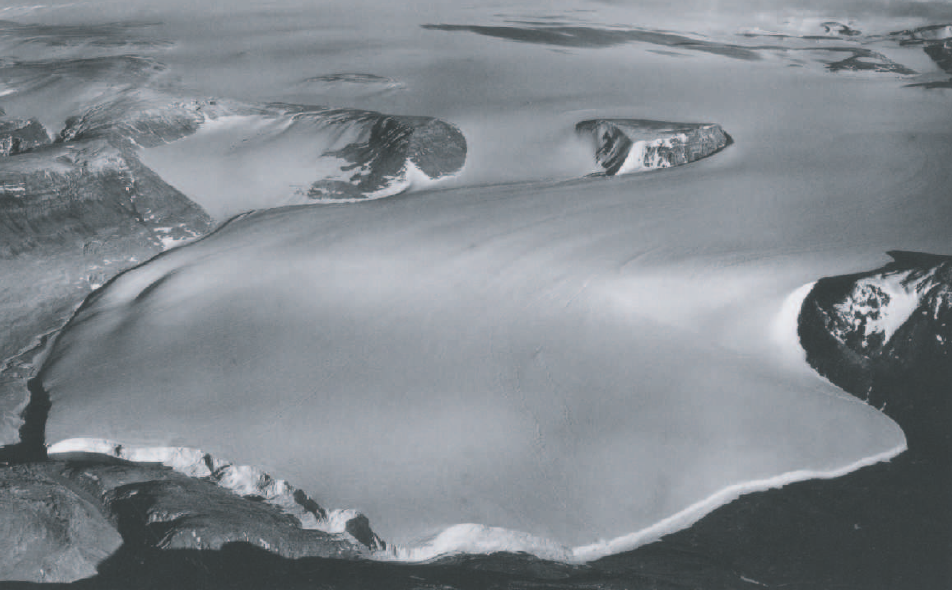
\includegraphics[width=1.0\textwidth]{polaris}
\end{column}
\begin{column}{0.35\textwidth}
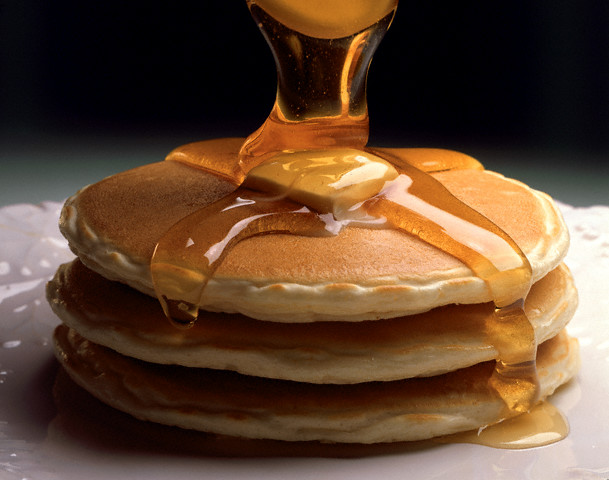
\includegraphics[width=1.0\textwidth]{pancakes}
\end{column}
\end{columns}

\bigskip
\begin{itemize}
\item glaciers and ice sheets are viscous flows at the large scale
  \begin{itemize}
  \item[$\circ$] at a smaller scale they are ice crystals
  \item[$\circ$] at yet-smaller scale they are molecules \dots atoms \dots quarks
  \end{itemize}
\item \emph{usage}: ``ice sheets'' are big, shallow glaciers
\end{itemize}
\end{frame}


\begin{frame}{ice sheets are shallow}

\begin{itemize}
\item cross section of Greenland ice sheet at $71^\circ$ N
  \begin{itemize}
  \item[$\circ$] {\color{dark green}{green}} and {\color{dark blue}{blue}}: vertically-exaggerated version
  \item[$\circ$] in {\color{dark red}{red}}: without vertical exaggeration
  \end{itemize}
\end{itemize}
\normalsize

  \begin{center}
    \tikz{\draw[<->] (0.0,-2.9) -- node [midway, left] {3500 m} (0.0,2.7);}  \quad 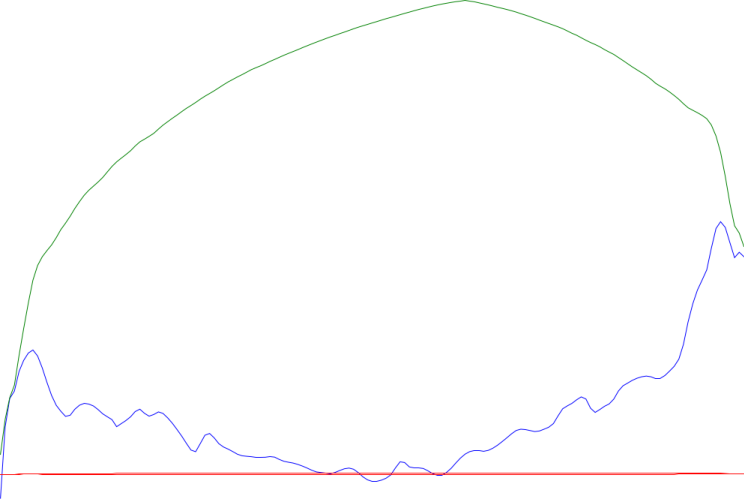
\includegraphics[width=0.7\textwidth]{greentransecttrimmed}
    
    \bigskip
    \qquad\qquad\qquad \tikz{\draw[<->] (-4.1,0.0) -- node [midway, below] {750 km} (4.1,0.0);}
  \end{center}
\end{frame}


\begin{frame}{what is a fluid?}

\begin{columns}
\begin{column}{0.6\textwidth}
\begin{itemize}
\item seriously, what is a fluid?
\item<2-> is it just a collection of particles?
\item<3-> a fluid is a mathematical abstraction
  \begin{itemize}
  \item<3->[$\circ$]   each smaller piece remains a fluid
  \item<3->[$\circ$]   a continuous function $y=f(x)$ is also such an abstraction
  \end{itemize}
\item<3-> a fluid is a \alert{model}
\item<4-> with primary variables:
  \begin{itemize}
  \item<4->[$\circ$]   velocity $\mathbf{u}(\bx,t)$
  \item<4->[$\circ$]   pressure $p(\bx,t)$
  \end{itemize}
\item<4-> gases, liquids, and \alert{ice} are all fluids (at big enough scale)
\end{itemize}
\end{column}
\begin{column}{0.4\textwidth}
\includegraphics<1>[width=\textwidth]{liquid}
\includegraphics<2>[width=\textwidth]{ivfluid}
\includegraphics<3>[width=\textwidth]{lighterfluidalpha}
\includegraphics<4>[width=\textwidth]{xinjiangglacier}
\end{column}
\end{columns}
\end{frame}


\begin{frame}{ice is a viscous fluid}

\begin{itemize}
\item these are fluids:
  \begin{itemize}
  \item[$\circ$] air
  \item[$\circ$] liquid water
  \item[$\circ$] syrup
  \item[$\circ$] glacier ice
  \end{itemize}
\item are usually modeled as \alert{incompressible viscous fluids}
\item a typical incompressible viscous fluid is described by Navier-Stokes equations:
\begin{align*}
\nabla \cdot \mathbf{u} &= 0 &&\qquad \text{\emph{incompressibility}} \\
\rho \left(\mathbf{u}_t + \mathbf{u}\cdot\nabla \mathbf{u}\right) &= -\nabla p + \nu \nabla^2 \mathbf{u} + \rho \mathbf{g} &&\qquad \text{\emph{stress balance}}
\end{align*}

\small
\item these equations are known to be hard
  \begin{itemize}
  \item[$\circ$] \$1 million Clay Institute prize for proving there are solutions in 3D \dots unclaimed for 18 years
  \item[$\circ$] but you've flown here on plane designed assuming we adequately understand them
  \end{itemize}
\end{itemize}
\end{frame}


\begin{frame}{ice is a weird viscous fluid}

\begin{itemize}
\item glacier ice is not a typical fluid!
\item for example, these are \alert{irrelevant in glacier flow}, but a big deal for weather and climate models of the atmosphere and ocean:
  \begin{itemize}
  \item[$\circ$] turbulence
  \item[$\circ$] convection
  \item[$\circ$] coriolis force
  \item[$\circ$] density variations
  \end{itemize}
\end{itemize}
\end{frame}


\begin{frame}{ice is a slow, shear-thinning fluid}

\begin{itemize}
\item recall Navier-Stokes:
\small
\begin{align*}
\nabla \cdot \mathbf{u} &= 0 &&\qquad \text{\emph{incompressibility}} \\
\rho \left(\mathbf{u}_t + \mathbf{u}\cdot\nabla \mathbf{u}\right) &= -\nabla p + \nu \nabla^2 \mathbf{u} + \rho \mathbf{g} &&\qquad \text{\emph{stress balance}}
\end{align*}
\normalsize
\item glacier ice fluid is
  \begin{enumerate}
  \item ``slow'' is a technical term:\footnote{the Froude number, the ratio of inertia to gravity, is approximately $10^{-15}$}

\vspace{-3mm}
    $$\rho \left(\mathbf{u}_t + \mathbf{u}\cdot\nabla \mathbf{u}\right) \approx 0 \qquad \iff \qquad \begin{pmatrix} \text{forces of inertia} \\ \text{are negligible} \end{pmatrix}$$
  \item non-Newtonian (shear-thinning):

    \begin{itemize}
    \item[$\circ$] viscosity $\nu$ is not constant
    \item[$\circ$] ``shear-thinning'' is a power law (Glen law):
        $$(\text{strain rate}) = A\, (\text{shear stress})^n$$
    \item[$\circ$] $1.8 < n < 4.0$ ?  \quad when in doubt: \alert{$n=3$}
    \end{itemize}
  \end{enumerate}
\end{itemize}
\end{frame}


\begin{frame}{equations for ice flow}

\begin{columns}
\begin{column}{0.65\textwidth}
\begin{itemize}
\item the \alert{standard model for ice flow} is Glen-Stokes:
\begin{align*}
\nabla \cdot \mathbf{u} &= 0 &&\text{\emph{incompressibility}} \\
0 &= - \nabla p + \nabla \cdot \tau_{ij} + \rho \mathbf{g} &&\text{\emph{stress balance}} \\
\mathbf{D}u_{ij} &= A \left|\tau_{ij}\right|^2 \tau_{ij} &&\text{\emph{Glen flow law}}
\end{align*}
\item notation:
  \begin{itemize}
  \item[$\circ$] $\tau_{ij}$ is deviatoric stress tensor
  \item[$\circ$] $\mathbf{D}u_{ij}$ is strain rate tensor
  \end{itemize}
\end{itemize}
\end{column}
\begin{column}{0.35\textwidth}

\hfill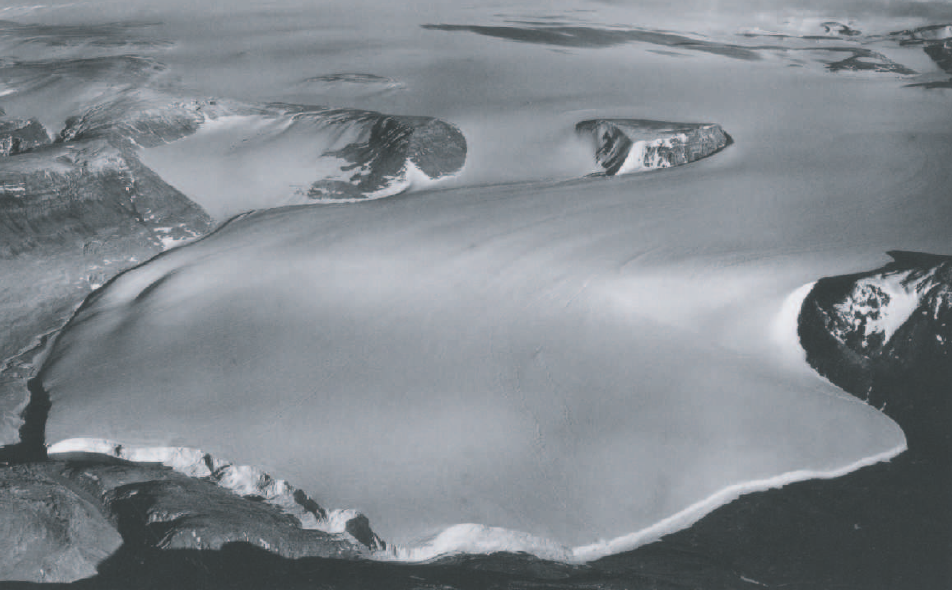
\includegraphics[width=0.9\textwidth]{polaris}

\bigskip\bigskip

\hfill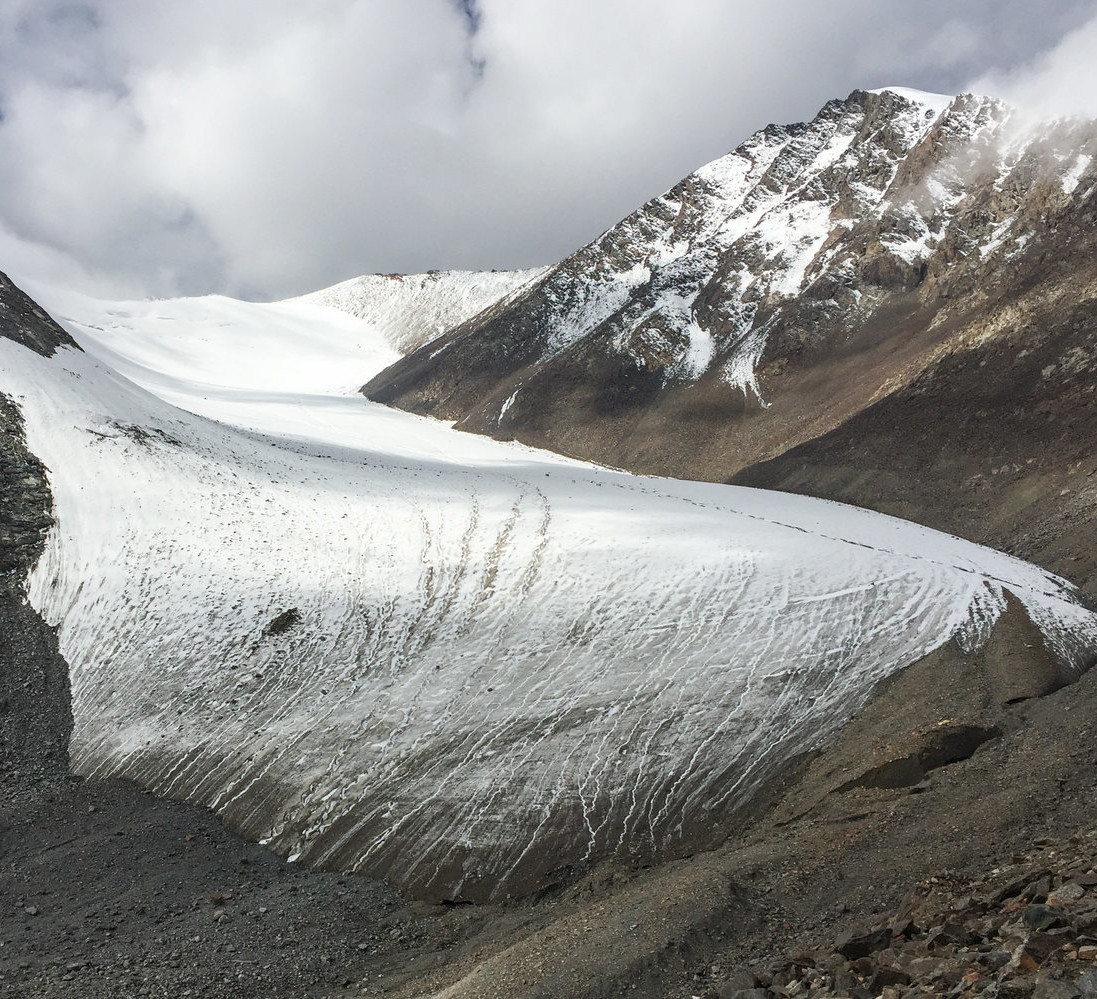
\includegraphics[width=0.9\textwidth]{xinjiangglacier}
\end{column}
\end{columns}
\end{frame}


\begin{frame}{wait \dots too many equations!}

\begin{itemize}
\item too many equations!
    \begin{itemize}
    \item[$\circ$] I know
    \end{itemize}
\item what math is needed for numerical models of fluids like glaciers?
    \begin{itemize}
    \item[$\circ$] calc III \hfill (\emph{partial derivatives, surface integrals, \dots})
    \item[$\circ$] linear algebra
        \begin{itemize}
        \item because pretty much the fanciest trick you can program on a computer is to solve a linear system $A\bx = \bb$
        \end{itemize}
    \item[$\circ$] differential equations \hfill (\emph{ODEs \emph{and} PDEs})
    \item[$\circ$] some computer programming
        \begin{itemize}
        \item Matlab or Python
        \item a course in numerical analysis is nice
        \end{itemize}
    \end{itemize}
\end{itemize}
\end{frame}


\section[big picture questions]{big picture questions for ice flow models}

\begin{frame}
  \frametitle{how much can sea level rise if ice sheets melt?}
  \framesubtitle{(big picture question 1)}

\begin{columns}
\begin{column}{0.6\textwidth}
\begin{itemize}
\item ice sheets are big masses of frozen water (mostly) sitting above the sea level
    \begin{itemize}
    \item[$\circ$] Greenland ice sheet mass is $2.9 \times 10^6$ Gt \quad $(\approx \text{km}^3)$ % = 2.93466 10^6 km^3  volume, from SeaRISE-Greenland 5km data
    \end{itemize}
\item if \emph{all} ice melts:
    \begin{itemize}
    \item[$\circ$] Antarctica: 61 m of sea level rise
    \item[$\circ$] Greenland: 7 m of sea level rise
    \item[$\circ$] all other glaciers: 35 cm of sea level rise
    \end{itemize}
\item so it would be good to know mechanisms of melt
\end{itemize}
\end{column}
\begin{column}{0.4\textwidth}

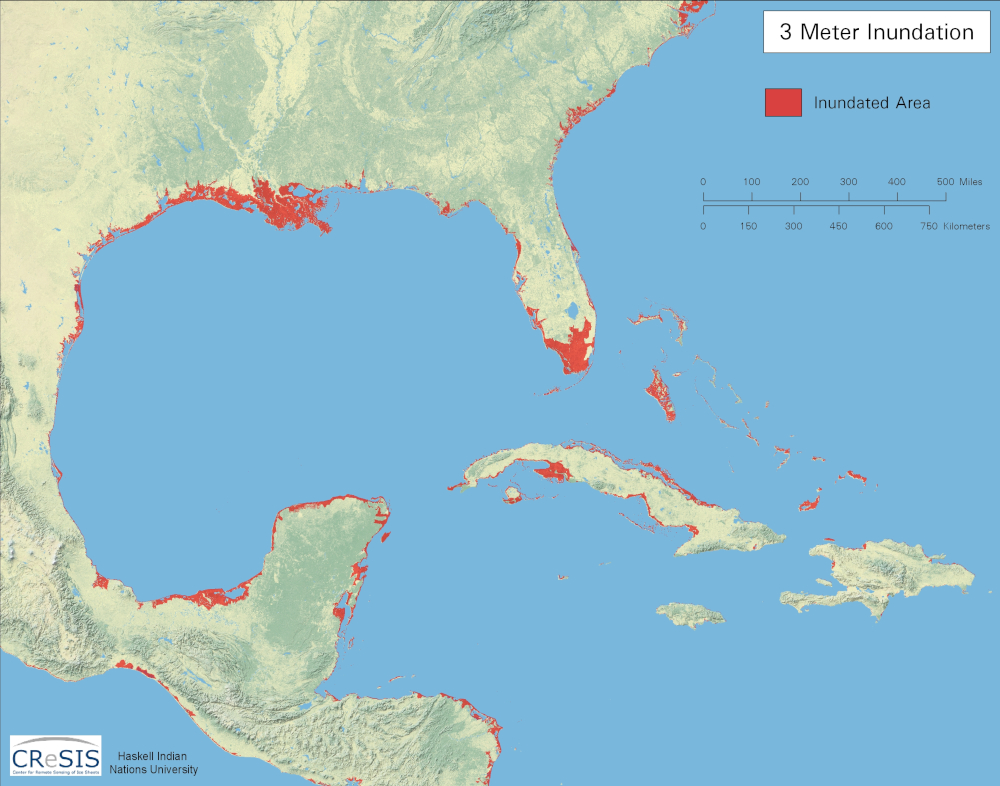
\includegraphics[width=0.95\textwidth]{southeastern_us_3m}
\end{column}
\end{columns}
\end{frame}


\begin{frame}
  \frametitle{how does flowing ice interact with climate?}
  \framesubtitle{(big picture question 2)}

\medskip
\small
\begin{itemize}
\item \emph{mass and energy inputs}: (1) snow adds, (2) sun heats, (3) ocean heats, (4) earth heats
\item \emph{mass outputs}: (1) surface meltwater, (2) basal meltwater, (3) ice discharge
\end{itemize}

\begin{center}
  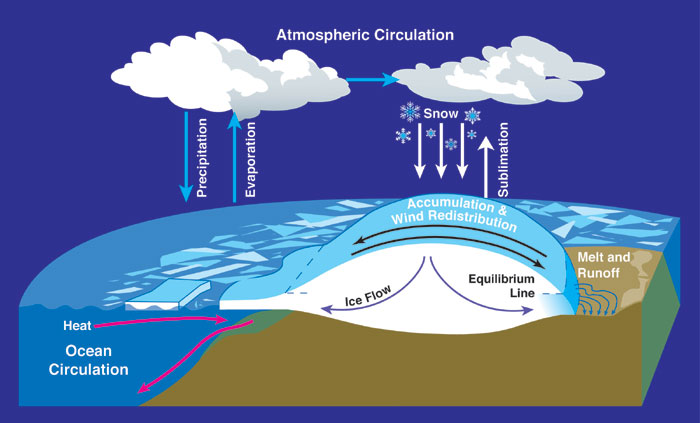
\includegraphics[width=0.75\textwidth]{mass-bal-atmos}
\end{center}
\end{frame}


\contactslipslide


\begin{frame}
  \frametitle{how to understand these viscous flows?}
  \framesubtitle{(big picture question 3)}

\begin{columns}
\begin{column}{0.6\textwidth}
\begin{itemize}
\item ice sheets are a separate category of fluid problems, worth studying
\item they have four outstanding properties \emph{as viscous flows}:
  \begin{enumerate}
  \item \alert{slow}
  \item \alert{shear-thinning}
  \item \alert{shallow}
  \item \alert{contact slip}
  \end{enumerate}
\item other fluids in same category:
  \begin{itemize}
  \item[$\circ$] salad dressing (\emph{look for ``xanthan gum'' as ingredient})
  \item[$\circ$] blood (\emph{except not shallow})
  \end{itemize}
\end{itemize}
\end{column}
\begin{column}{0.4\textwidth}

\hfill 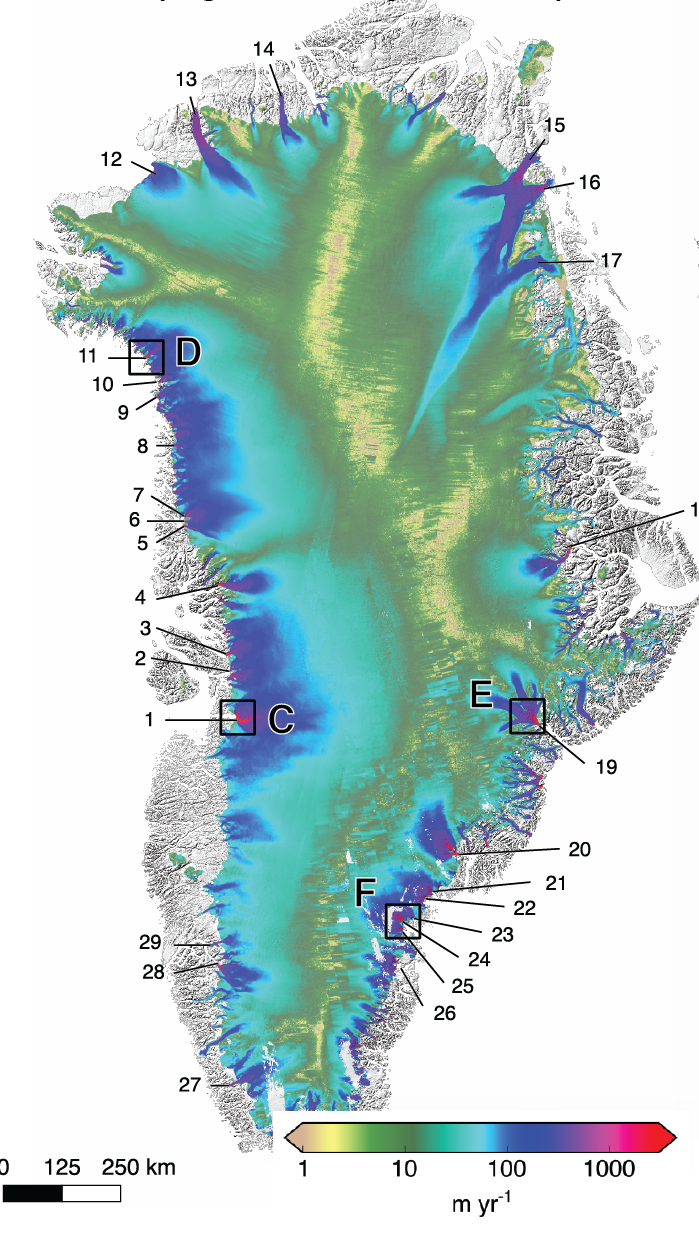
\includegraphics[width=0.95\textwidth]{greenland-overview-obsonly}
\end{column}
\end{columns}
\end{frame}


\section[numerical models]{numerical models of ice sheets}


\begin{frame}
  \frametitle{the main variables in a model}

\begin{center}
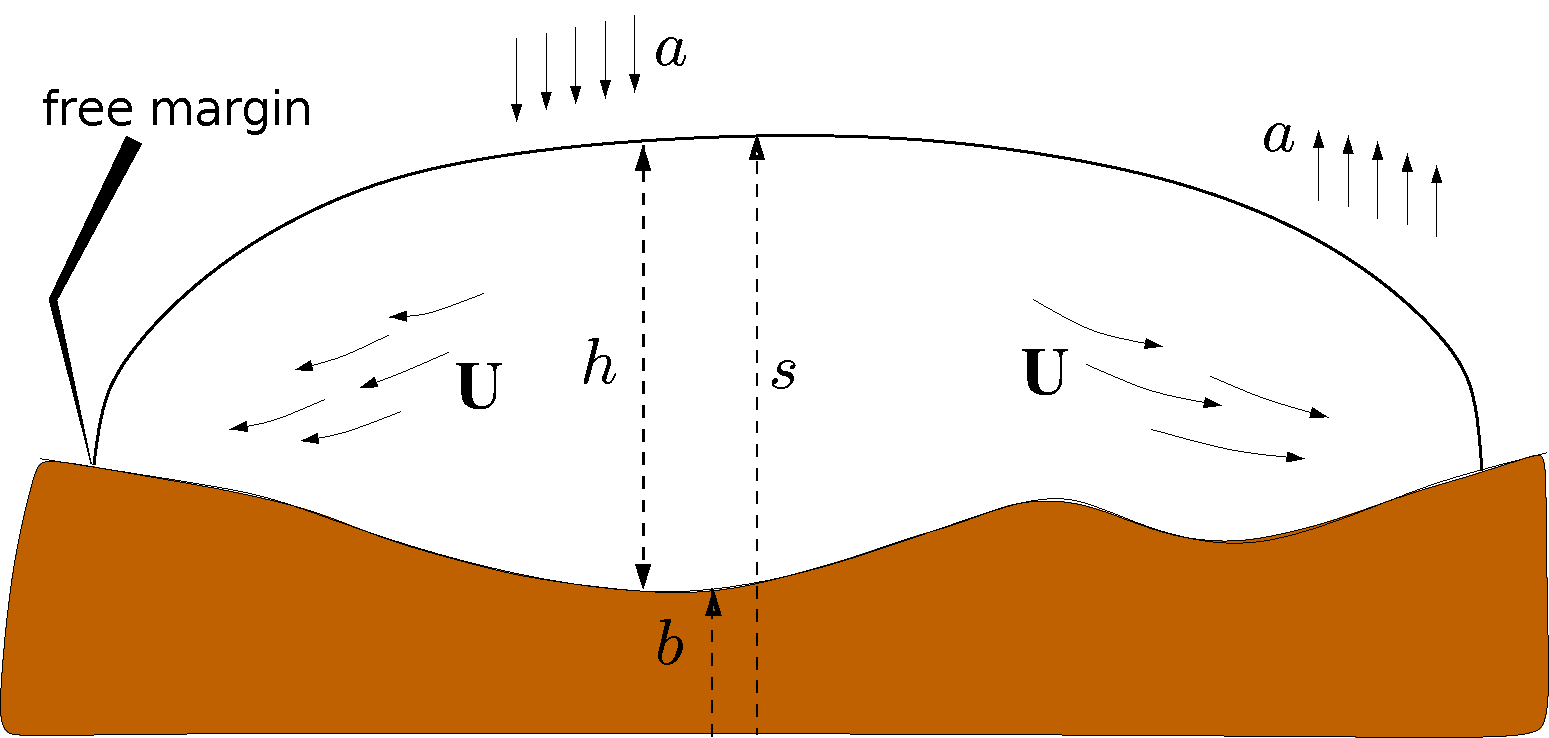
\includegraphics[width=0.7\textwidth]{groundedscheme}
\end{center}

\begin{itemize}
\small
\item $s=$ ice surface elevation
\item $b=$ bedrock elevation
\item $h=$ ice thickness $ = s-b$
\item ${\bf u}=$ velocity field
\item $a=$ surface mass balance (accumulation)

\bigskip
\item obvious(?) idea: ice surface $s$ is always above the bedrock $b$
\end{itemize}

\end{frame}


\begin{frame}
  \frametitle{a mathematical modeling analogy}

\begin{columns}
\begin{column}{0.35\textwidth}
\begin{itemize}
\item ice sheet surface \\ = \alert{membrane}
\item bedrock = \alert{obstacle}
\end{itemize}
\vfill
\begin{center}
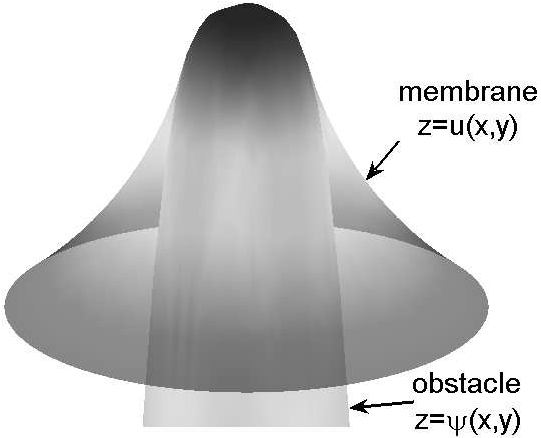
\includegraphics[width=1.1\textwidth]{classicalobs}
\end{center}
\end{column}
\begin{column}{0.65\textwidth}
\begin{center}
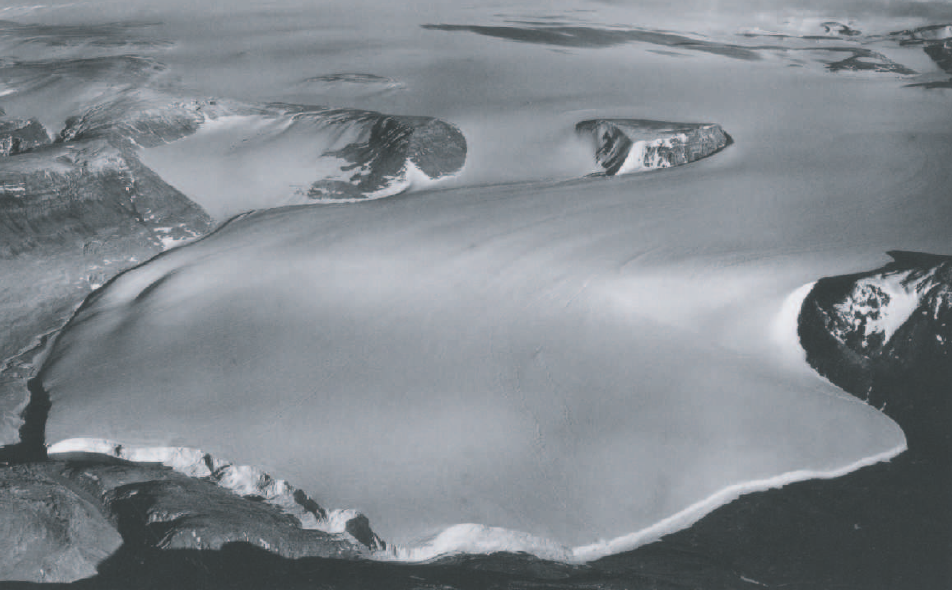
\includegraphics[width=0.8\textwidth]{polaris} \\
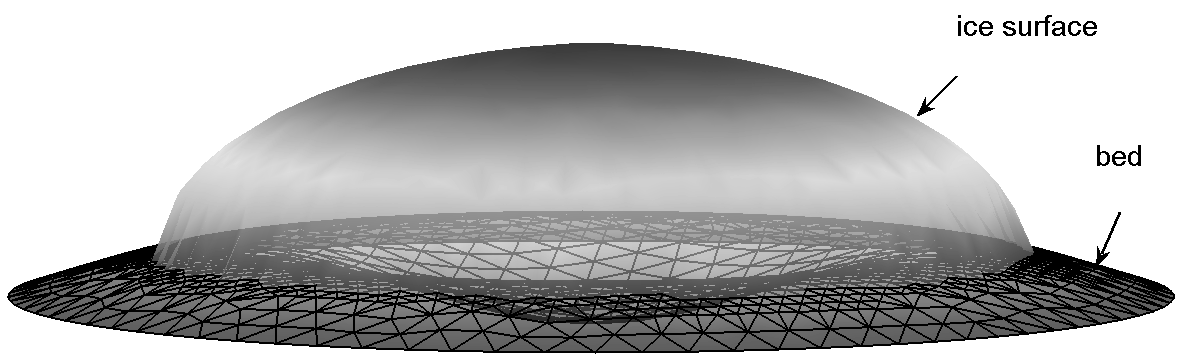
\includegraphics[width=\textwidth]{capnonflatobs}
\end{center}
\end{column}
\end{columns}
\end{frame}



\begin{frame}
  \frametitle{shallow ice approximation (SIA)}

\begin{itemize}
\item recall standard Glen-Stokes model:
\small
\begin{align*}
\nabla \cdot \mathbf{u} &= 0 &&\text{\emph{incompressibility}} \\
0 &= - \nabla p + \nabla \cdot \tau_{ij} + \rho \mathbf{g} &&\text{\emph{stress balance}} \\
\mathbf{D}u_{ij} &= A \left|\tau_{ij}\right|^2 \tau_{ij} &&\text{\emph{Glen flow law}}
\end{align*}
\normalsize
\item SIA is good approximation of standard model when
  \begin{itemize}
  \item[$\circ$] sliding is small or zero
  \item[$\circ$] bedrock slope is modest
  \end{itemize}
\item derive SIA equations by scaling Stokes based on shallowness:
  \begin{itemize}
  \item[$\circ$] $[h]$ is a typical thickness, $[x]$ is a typical width
  \item[$\circ$] small parameter is $\eps = [h] / [x]$
  \end{itemize}
\item horizontal ice velocity is given by ($n=3$): 
  $${\bf U}  =  - \frac{2 A}{4} (\rho g)^{3} \left[ (s-b)^4 - (s - z)^4  \right] 
|\nabla s |^{2} \nabla s$$

\vspace{-2mm}
  \begin{itemize}
  \item[$\circ$] no PDE to solve for velocity
  \end{itemize}
\end{itemize}
\end{frame}



\begin{frame}
  \frametitle{steady state}

\begin{itemize}
\item mass conservation in steady state: 
  $$\Div \left(  \int_b^s {\bf U}\, dz \right)  =  a$$
\item shallow ice approximation + (steady) mass conservation:
\begin{equation}
- \Div \left(\Gamma (s-b)^5 | \nabla s |^2 \nabla s  \right) =  a  \tag{$\ast$}
\end{equation}
  \begin{itemize}
  \vspace{-0.2in}
  \item[$\circ$] this is the major SIA equation \dots a PDE
  \item[$\circ$] the unknown is ice surface elevation $s(x,y)$
  \item[$\circ$] like Poisson equation $-\Div (\nabla u) = f$ except nonlinear and singular
  \end{itemize}
\item the most basic numerical ice sheet model is a program which approximately solves ($\ast$) for $s(x,y)$ given steady climate inputs $a(x,y)$ and bed elevation $b(x,y)$
\end{itemize}
\end{frame}


\begin{frame}{movie of time-dependent SIA}

\begin{columns}
\begin{column}{0.4\textwidth}
\small
\begin{itemize}
\item at right is the Halfar similarity solution
\item an exact, time-dependent, zero mass balance solution where the $t\to 0^+$ limit is a delta function
\item compare Barenblatt solution of porous medium equation
\end{itemize}
\end{column}

\begin{column}{0.65\textwidth}
\vspace{-0.25in}

\begin{center}
\animategraphics[autoplay,loop,height=4.7cm]{4}{../commonfigs/animhalfar/halfar}{0}{26}

\bigskip
\tiny
frames from $t=4$ months to $t = 10^6$ years,

equal spaced in \emph{exponential} time
\end{center}
\end{column}
\end{columns}
\end{frame}


\contactslipslide


\begin{frame}
  \frametitle{ice shelf versus sea ice}

\begin{center}
\vspace{-0.2in}

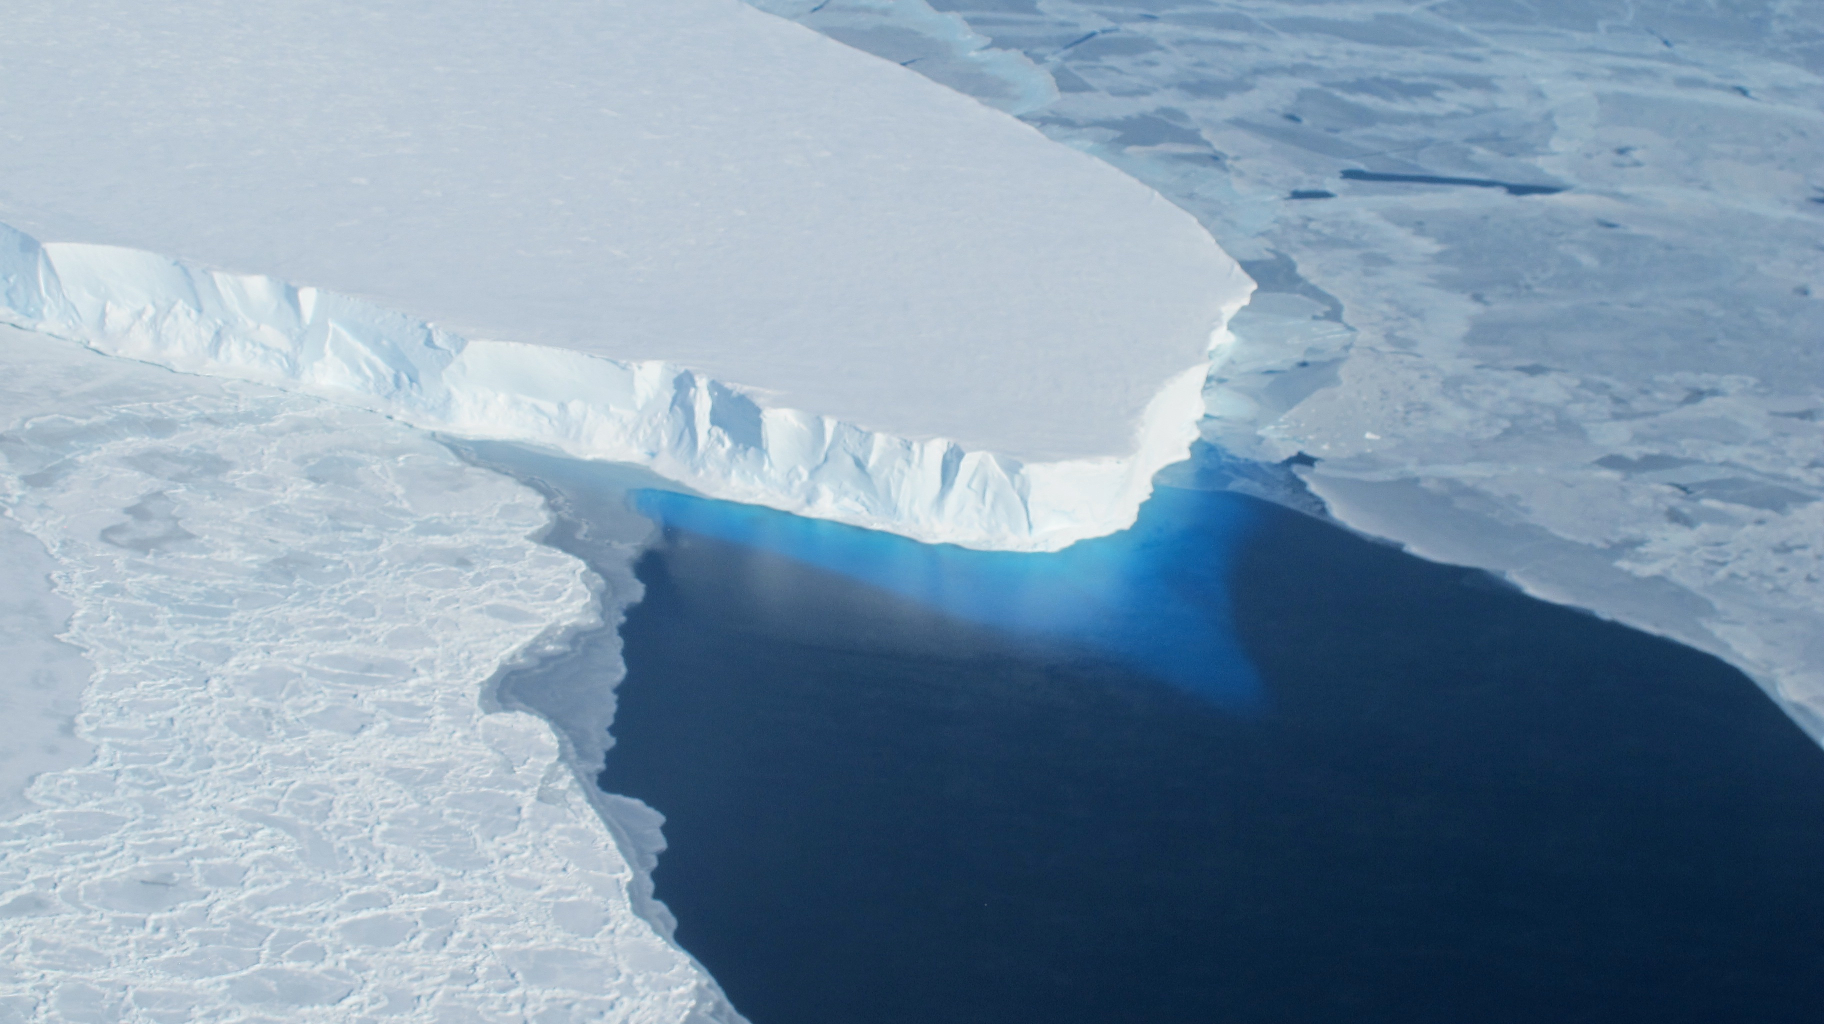
\includegraphics[width=1.0\textwidth]{supp4rignot-small}

\medskip
\tiny [ice shelf at Thwaites Glacier, Antarctic]
\end{center}
\end{frame}


\begin{frame}{models of ice shelves: they work}

\begin{itemize}
\item Ross ice shelf (Antarctica) velocity below
  \begin{itemize}
  \item[$\circ$] observed versus computed by SSA model in PISM
  \item[$\circ$] tuned: single, constant $A$
  \end{itemize}
\end{itemize}
\vspace{-0.3in}

\begin{center}
  \mbox{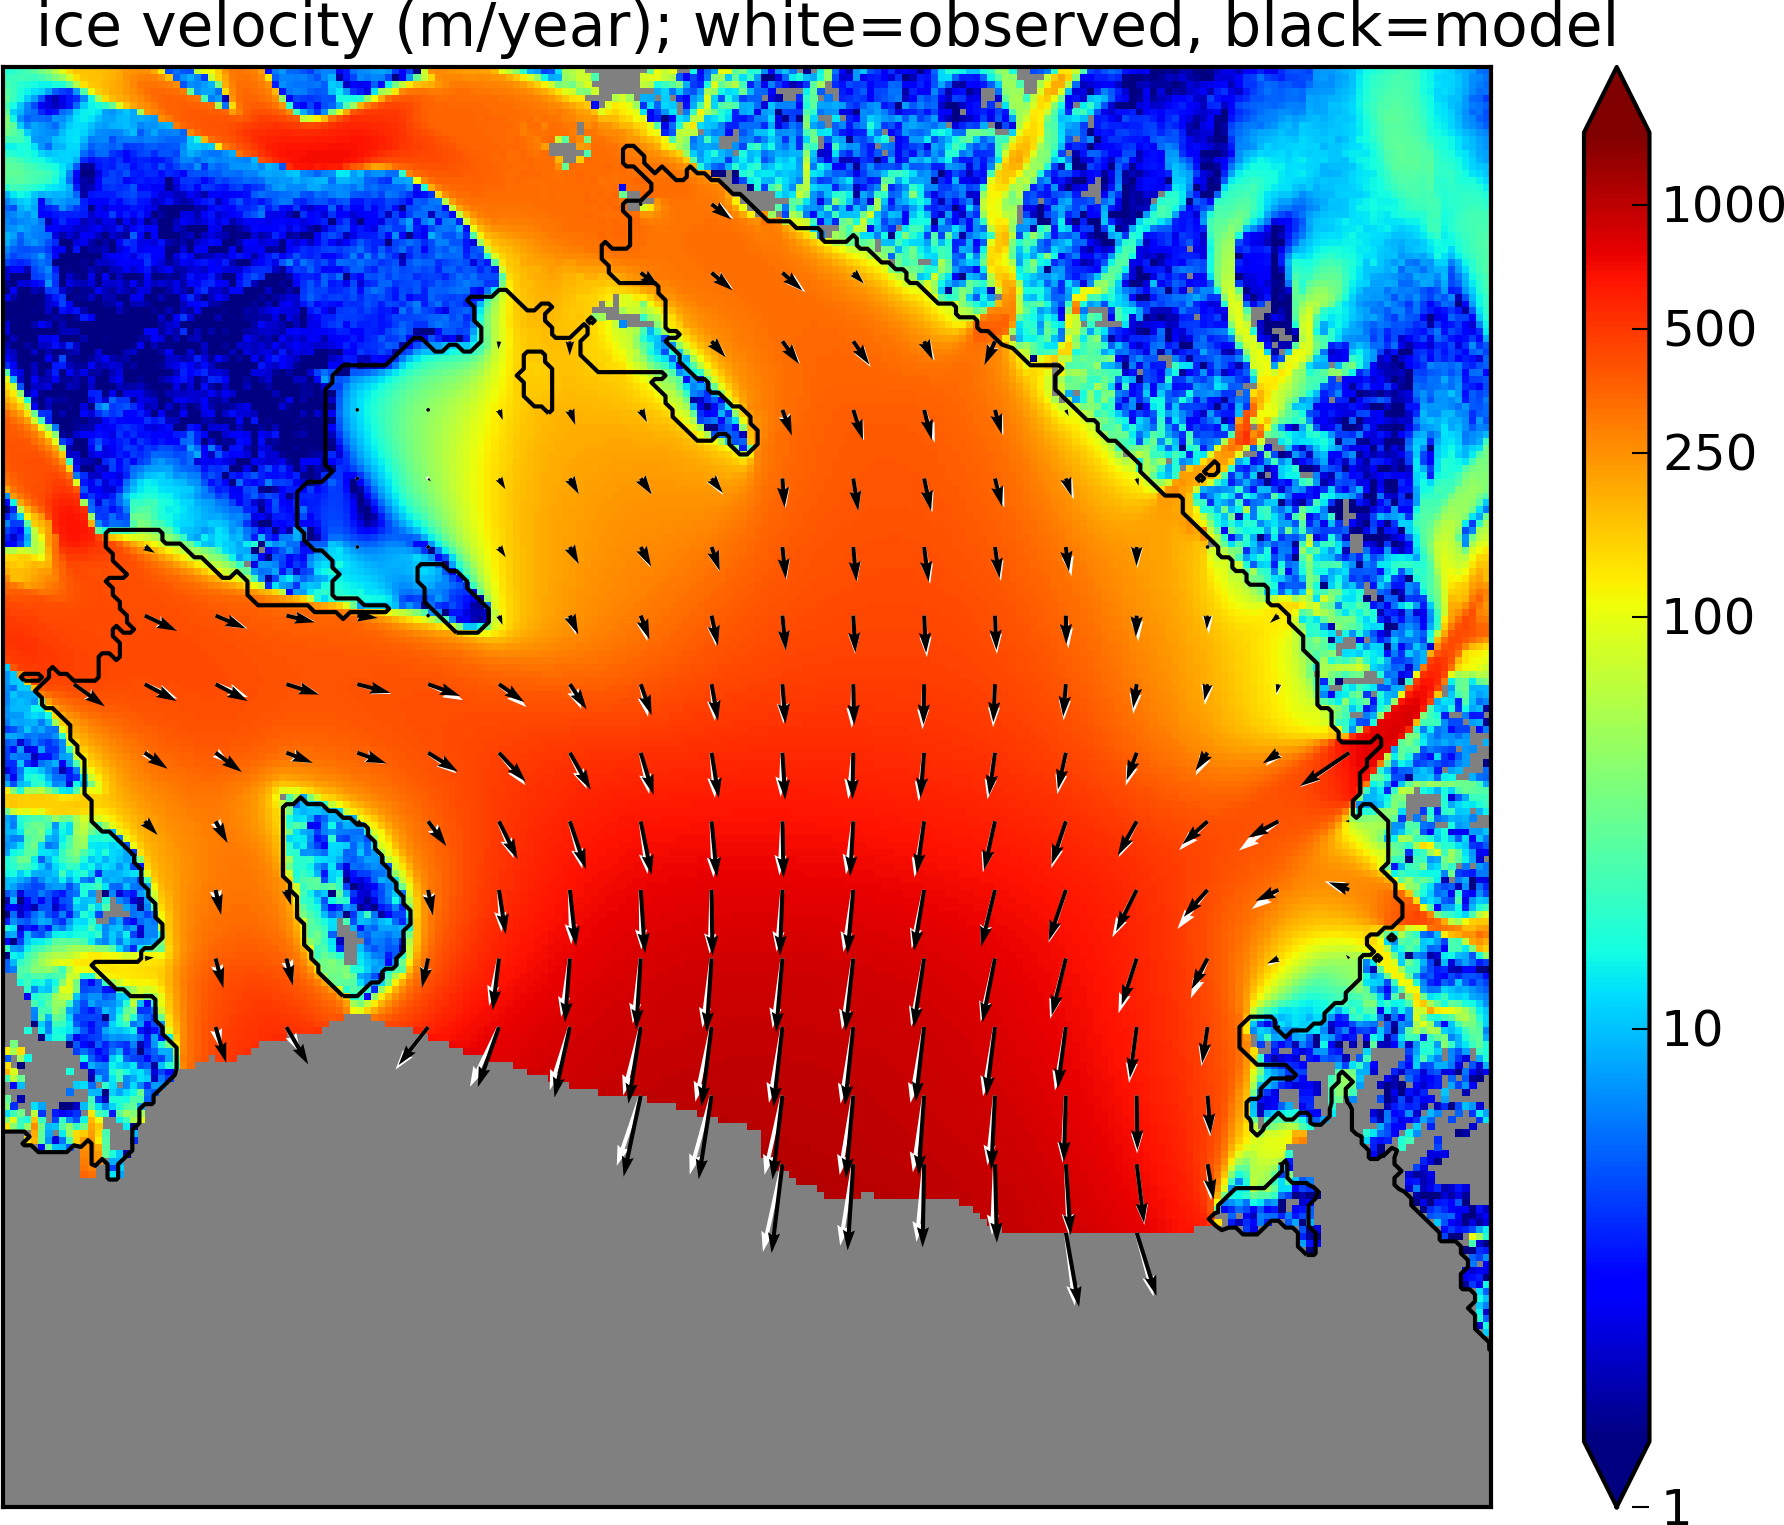
\includegraphics[width=0.58\textwidth]{rossquiver} \, 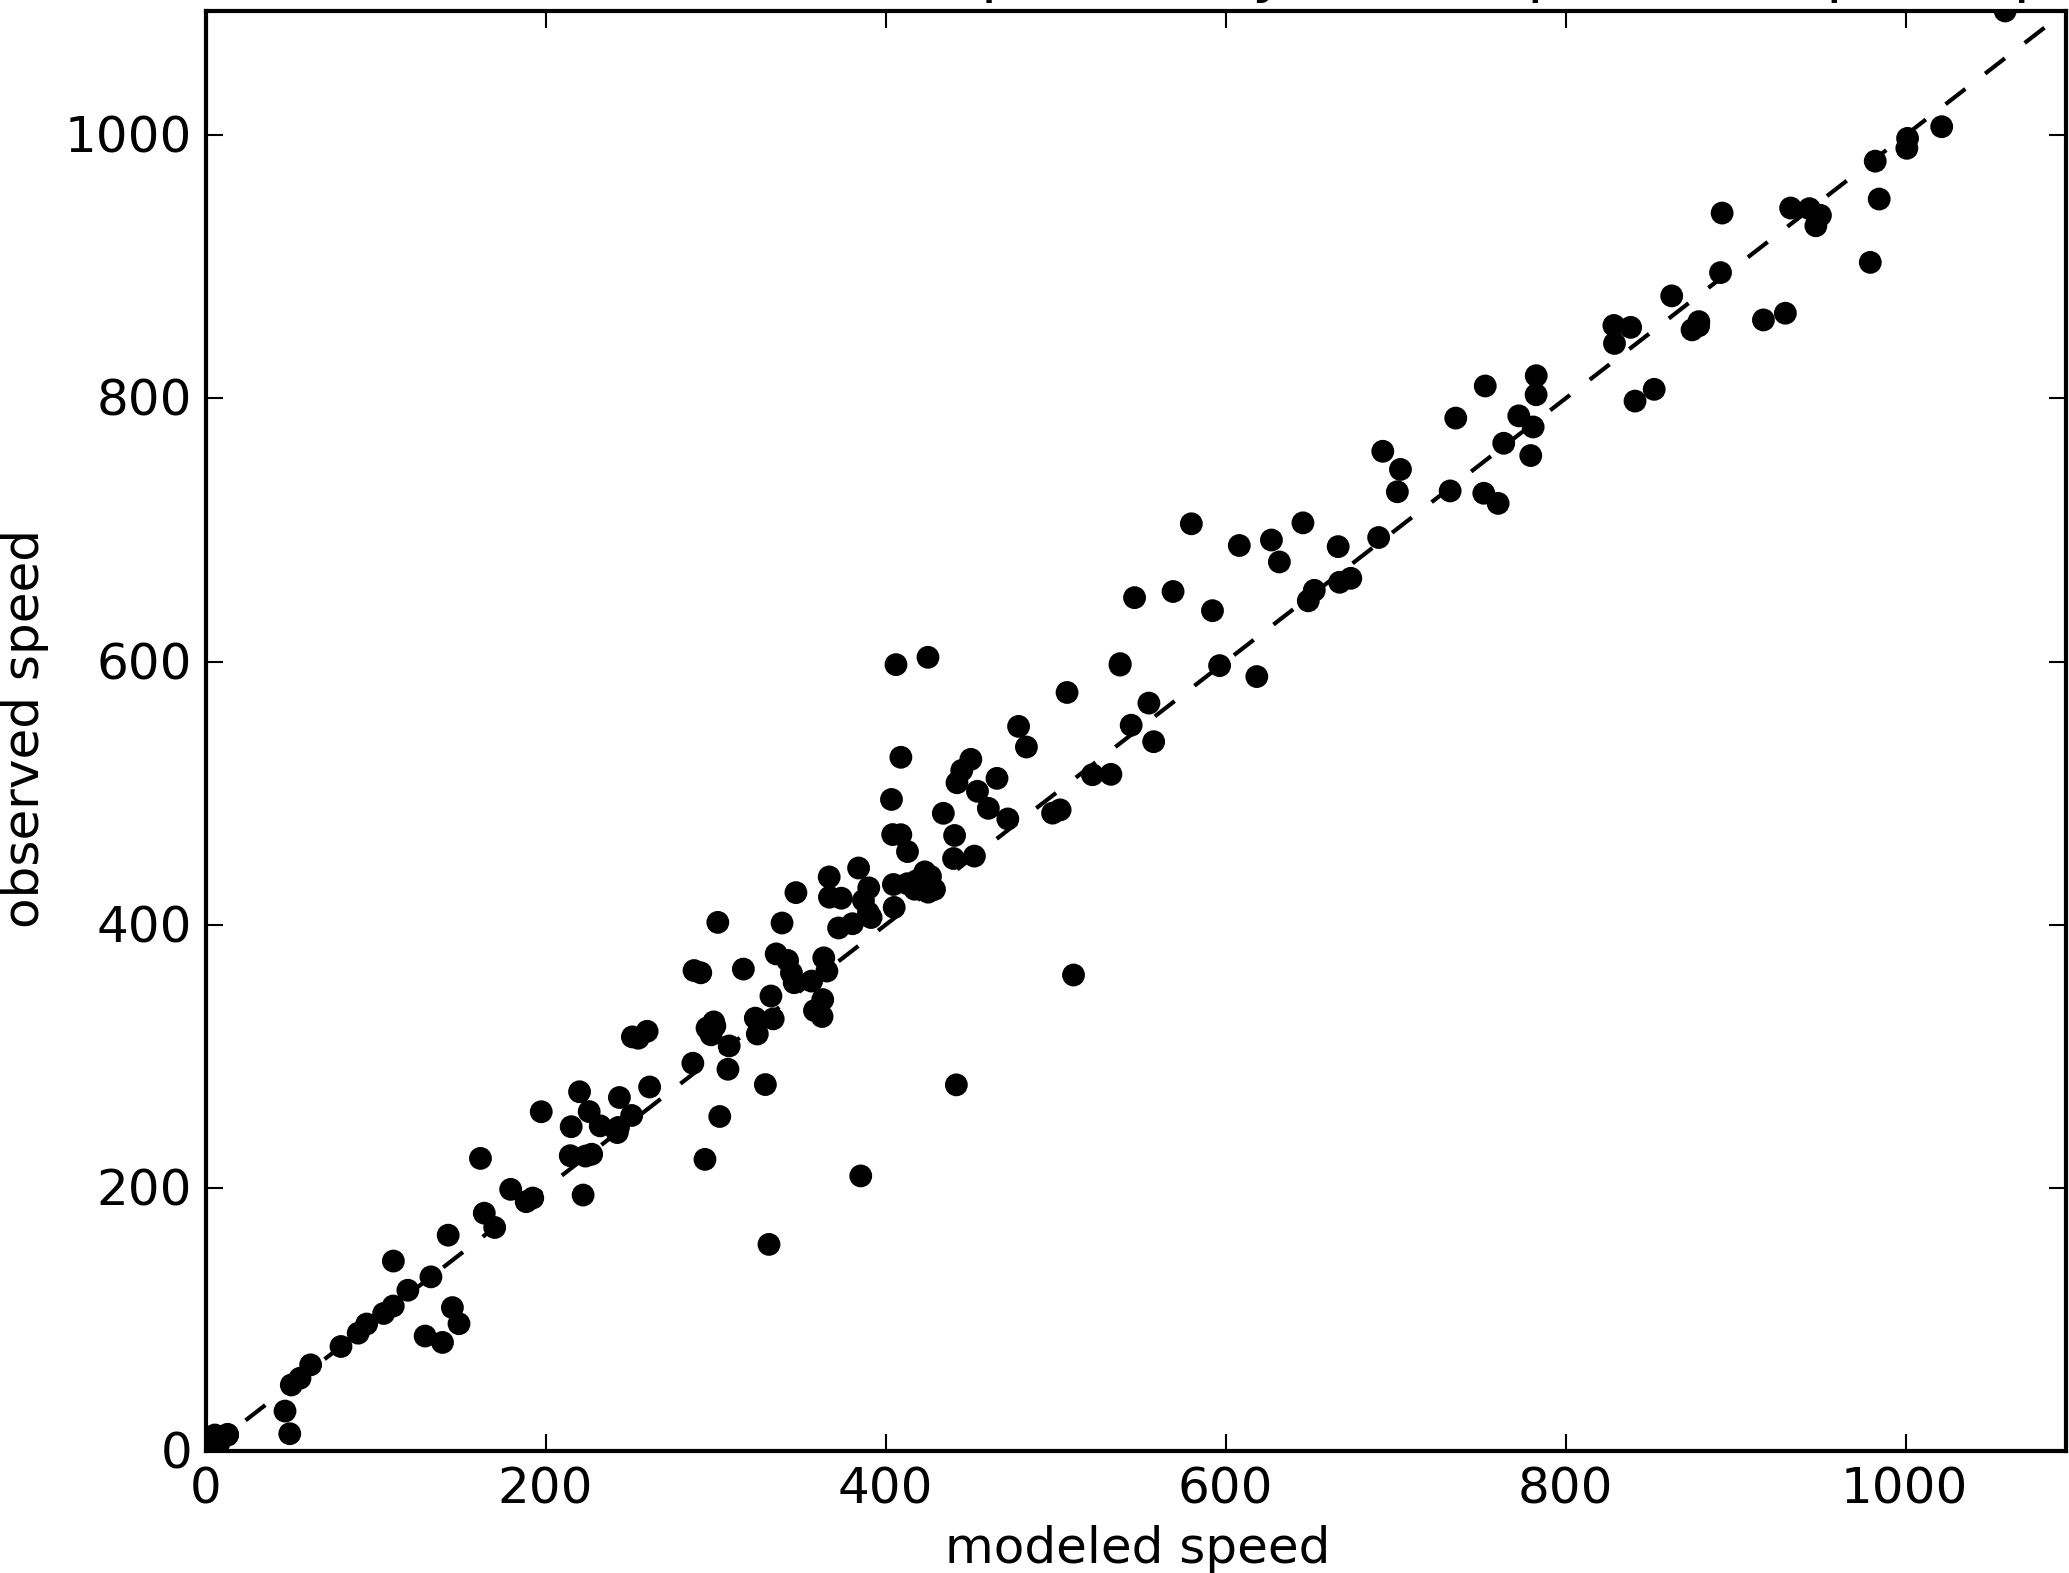
\includegraphics[width=0.48\textwidth]{rossscatter}}
\end{center}
\end{frame}


\begin{frame}
  \frametitle{ice streams: an analogy}

\begin{columns}
\begin{column}{0.6\textwidth}
\begin{itemize}
\item ice shelves have zero basal resistance
\item ice streams emerge where basal resistance is low enough
\item basal resistance is low if there is pressurized liquid water underneath the ice sheet
\item ice sheet is a membrane which connect sliding ice to upstream and/or lateral non-sliding ice
\end{itemize}
\end{column}
\begin{column}{0.4\textwidth}
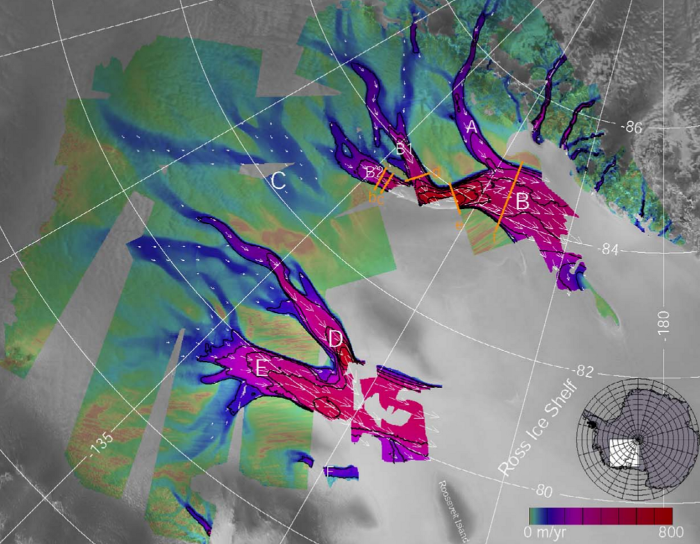
\includegraphics[width=\textwidth]{siple}

\vspace{0.3in}

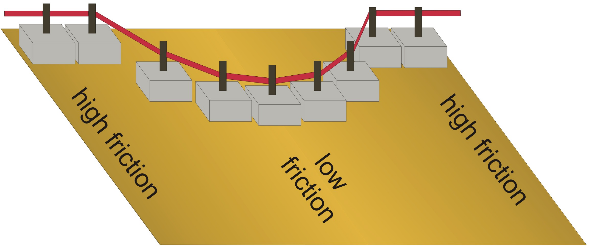
\includegraphics[width=1.1\textwidth]{schoof-sliders}
\end{column}
\end{columns}
\end{frame}

\begin{frame}{numerical model results}

FIXME show Andy RPC greenland results movie
\end{frame}


\section[on being right]{how do we know the numerical models are right?}

\begin{frame}
  \frametitle{moving grounding line in the lab}
  \framesubtitle{by Pegler et al.~(2014)}

\begin{center}

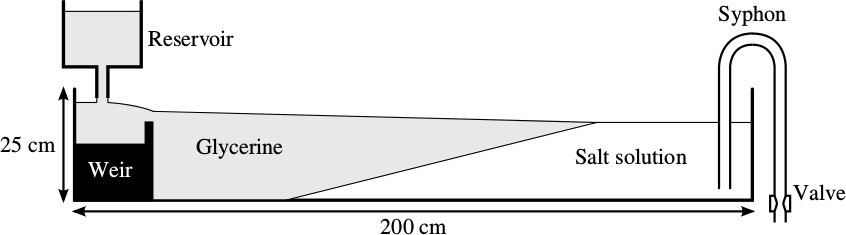
\includegraphics[width=0.7\textwidth]{pegler2014-grounding-line-schematic}

\vspace{1.0in}
[show movie]
\end{center}
\end{frame}


\begin{frame}{FIXME slide about exact solutions}
\end{frame}


\begin{frame}{FIXME slide about MMS}
\end{frame}



\section*{conclusion}

\begin{frame}
  \frametitle{conclusion}
  \framesubtitle{thanks for listening!}

\begin{center}
FIXME
\end{center}

\end{frame}


\end{document}
